\documentclass[a4paper,twoside]{article}

\usepackage{epsfig}
\usepackage{subcaption}
\usepackage{calc}
\usepackage{amssymb}
\usepackage{amstext}
\usepackage{amsmath}
\usepackage{amsthm}
\usepackage{multicol}
\usepackage{pslatex}
\usepackage{apalike}
\usepackage{verbatim}
\usepackage{float}
\newcommand{\myfloatalign}{\centering}
\usepackage[ruled]{algorithm2e}
\usepackage{graphicx,color,url}
\usepackage{SCITEPRESS}     % Please add other packages that you may need BEFORE the SCITEPRESS.sty package.


\begin{document}

\title{Speeding up evaluation of structures for the Angry Birds Game}

\author{\authorname{First Author Name\sup{1}\orcidAuthor{0000-0000-0000-0000}, Second Author Name\sup{1}\orcidAuthor{0000-0000-0000-0000} 
and Third Author Name\sup{2}\orcidAuthor{0000-0000-0000-0000}}
\affiliation{\sup{1}Place Holder, XYZ University, My Street, MyTown, MyCountry}
\affiliation{\sup{2}Place Holder, Main University, MySecondTown, MyCountry}
\email{\{f\_author, s\_author\}@ips.xyz.edu, t\_author@dc.mu.edu}
}

\keywords{Search-Based Procedural Content Generator, Evolutionary algorithm, 
Game development, Angry Birds, Level generation }

\abstract{
	In this work, we present an original method based on evolutionary algorithms for generating basic structures for the physics-based game Angry Birds, with the ultimate objective of creating Angry Birds levels with the minimum number of constraints. We set out to evolve free-form structures, and this means searching in a larger space. In this paper, we test how using a physics engine enables us to evaluate much more levels than a game engine simulation. In order to do this, we compare the results of experiments using both types of simulators and propose fitness functions accordingly. Results show the execution time drastically drops from 5 hours to less than 20 minutes on average. 
}

\onecolumn \maketitle \normalsize \setcounter{footnote}{0} \vfill

\section{\uppercase{Introduction}}
\label{sec:intro}
\textit{Angry Birds} is a multiplatform video game created in 2009 by
the Rovio Entertainment  Corporation. Each level of the game consists
of a collection of structures made out of blocks in which comic  {\em
  pig} characters are hiding;  the player has to fire from a slingshot
different {\em bird} characters, each having different abilities and
moods.  The objective of the game is to destroy all the pigs by
knocking down the structures or just hitting them directly.  The game
relies on gravity to create interesting puzzles by closely resembling
the dynamics of real-world structures. It has been approached in
different ways from the computational intelligence community; in this
paper we are interested in generating levels that are playable and
interesting. This has been proposed as a competition in several
game-related conferences
\cite{AngryBirds_LevelGeneration_18,GAIG_LevelGeneration_18}, but
could be also interesting from the perspective of generating levels
to train or evaluate game-playing bots, as was done by Zafar et al. in
\cite{zafar2019corpus}.

Search-based Procedural Content Generation (SBPCG) is a type of a
\textit{generate-and-test} approach to PCG which is usually tackled
with Evolutionary Algorithms(EA) \cite{togelius2010search}. The
challenges faced by SBPCG are not far from those found in EAs; since
they are search methods, they can be a good option to implement this
kind of systems. In our case, as a first step to generate Angry Birds
levels, we will generate free-form self-standing structures using the Angry
Birds basic blocks. The main intention with this approach is to
eventually generate structures that can host {\em pigs} and that
achieve aesthetic quality mainly through variability and the fact that
they are not cookie-cutter repetitions of the same basic structure
with some small variations; at the same time,
it becomes an interesting and challenging problem from the
optimization point of view: using some basic building blocks and a
simulated gravity, to be able to generate structures that do not
collapse. That is the main objective of this line of work.

The primary objective of this paper, however, is to use a fitness function that is
able to evaluate structures without needing the simulator, advancing
the state of the art with respect to our previous paper
\cite{DBLP:conf/evoW/CalleGGV19anon}, where we needed to use the simulator
itself to check gravity, which incurred in much overhead, up to
several seconds.

In this paper, we will use what \cite{togelius2010search} calls {\em
  direct fitness function}, this function computes a score from
measurable features of the generated content. However, this fitness
function is a time-consuming task since it involves the generation of
a graphic representation of the structure and the simulation of the
falling motion. If we have to evaluate every single individual in the
population, we will not be able to cover enough of the free-form
search space to find a good enough solution. So we must minimize the
actual number of structures that are simulated by applying heuristics
to the data structure and assigning it a fitness even before the
simulation. Additionally, we will try to improve the design of the
fitness function so that it does not focus only on creating stable
structures, but also structures that have a better appearance and
aesthetics. 


This paper is organized as follows: in the next section, we present
the state of the art in this type of level generation, as well as its
relation to the problem of generating structurally sound
structures. Our proposed method for generating Angry Birds levels is
described next in Section \ref{sec:angry}. The new experiments
performed for this paper and its results are presented next in section
\ref{ch:res}. We present our conclusions in 
\ref{sec:conclusions}.


\section{Background and State of the Art}
\label{sec:soa}

PCG used for video game levels is relevant in international artificial
intelligence competitions, such as Super Mario Level Generation
\cite{MarioAI_Level_12}, General Video Games
\cite{GAIG_LevelGeneration_18,Khalifa_GVGLG_16}, or recently, for
Angry Birds \cite{AngryBirds_LevelGeneration_18}. This work is related
to works presented in previous editions of the competition.  The focus
of the latest edition \cite{AngryBirds_LevelGeneration_18} was on
finding entertaining levels. Fun was the main factor in the evaluation
of proposals; secondary factors were creativity and difficulty.  Six
entries participated, of which J. Yuxuan et al., were able to generate
random quotations with different components of a level; J. Xu et
al. generated levels that look like pixel images. A third approach (by
C. Kocaogullar) translated music patterns to generate structures. The
winner was {\em Iratus Aves}, a new iteration of the work by M. Stephenson
and J. Renz \cite{stephenson2017generating,stephenson2016procedural},
which follows a \textit{constructive method}. In this work, the
likelihood of selecting a certain block is given by a probability
table, which was tuned using an optimization method. Blocks are then
stacked following a tree structure.

A constructive method ensures local stability, but not global
stability, which must be evaluated once the whole structure is
completed. One problem with this and other constructive approaches is
that the variety of structures created is going to be relatively
small; monotony leads to boredom, decreasing playability. On the other
hand, generated structures are guaranteed to be structurally sound,
and constructive approaches are generally faster than search-based
procedures. 


An alternative to deal with these limitations is to follow a
\textit{Search-based approach}. Thus, Lucas Ferreira and Claudio
Toledo \cite{ferreira2014search,Ferreira2014ASA} presented a solution using a Genetic
Algorithm (GA) and a clone of Angry Birds named \textit{Science Birds} developed
to evaluate the levels. In this GA, levels correspond to
individuals in a population, each individual has a chromosome
represented by an array of lists. Each list is a sequence of blocks,
pigs and predefined compound blocks, using an identification
number. Each list is then placed as a stack of elements in the game. A
level has several such stacks. This representation also includes the
distances between stacks. The population is initialized randomly
following a probability table defining the likelihood of a certain
element being placed in a certain position within a stack. This
implies that a column or stack shape is chosen beforehand, once again
ensuring stability, but decreasing playability by generating
structures whose only differences are which blocks are placed on top
of which. 

Levels are evaluated executing them in the simulator and checking
their average stability, considering the speed of every block when
erected -- which must tend to be zero when having a stable structure
--. The authors designed specialized crossover and mutation operators,
aiming to maintain the consistency of newly generated solutions.

The approach proposed by Stephenson et al. \cite{stephenson2019agent}
is based on agents, and is focused on offering custom experience for
specific players. This approach builds on the previous paper
\cite{Stephenson2018DeceptiveAB}, which tries to create {\em
  deceptive} levels that are able to minimize damages to the structure
in sequences of shots. Although the focus of this paper is in another
different direction, our constructive approach to design levels could
be complemented with different fitness scores, such as the ones
presented in Stephenson's papers.

However, this work proposes a different approach: \textit{free-form
  evolution}.  If we look outside the domain of game development and
focus on structural optimization in architecture, there are several
proposals using search-based algorithms. We can find a metaheuristic
called Cuckoo Search \cite{gandomi2013cuckoo} which performance was
tested with structural optimization. However, this optimization is
heavily parametrized and we are looking for the evolution of
structures that do not follow a predefined pattern.  Another approach
for structure design is using Generative Grammatical Encodings
\cite{hornby2001advantages} where L-system and its production rules
are considered individuals. This method increases the number of
generated patterns,  but still restrains the formation of disjoint
structures, for instance, a defensive tower before a simple pigsty in
our context. 

We aim at following a realistic structure generation approach, without
constraining it to a fixed form, thus advancing the state of the art
by allowing the creation of Angry Birds levels having any
arrangement. The next section will describe how we characterize this
problem and our approach to it. In our previous paper
\cite{DBLP:conf/evoW/CalleGGV19anon} we explored this approach and found
as one of its shortcomings the fact that the evaluation of generated
structures through the simulator was lengthy and didn't leave the
algorithm enough time to explore the search space. In this paper, we
try to tackle that problem, as well as take additional steps to
increase the complexity of generated structures. 

\section{Problem Description}
\label{sec:angry}

In a previous work, we used {\em Science Birds}
\cite{ferreira2014search}  as a starting point. Developed by Lucas
Ferreira and Claudio Toledo, Science Birds has become the main open
source Angry Birds simulator. However, we needed to modify the code in
order to produce an output with the additional data needed to automate
that work. The code is available in the GitHub repository
% \url{https://github.com/Laucalle/ScienceBirds}
\url{https://url.hidden}
. The additional data
contains the position and the average magnitude of the velocity of
each block that remains after the simulation. One advantage is that
the whole experiment can run without user intervention. Another
advantage is that the amount of time spent on the simulation of each
level is minimized to some extent.  Reducing the simulation time not
only increases the number of evaluations by a certain range of time,
but it is also a factor in competitions, where there is a fixed time
limit for participants. 


To further decrease simulation time, in this paper, we use the Box2D
(\url{https://box2d.org}) physics engine. This engine, written in C++,
was initially used for the actual Angry Birds game. By just simulating
the positioning of objects in memory, we can avoid launching the whole
game, using bitmaps and screen rendering, which adds overhead to the
process of fitness evaluation. Even if in this Box2D simulation we do
not have the resistance of the blocks implemented, we can test the
stability of level much more efficiently, since there is no overhead
in computing things unrelated to Physics, such as the GUI. If we do
not have block resistance in a simulation, blocks will not be
destroyed when they hit each other; in that case, the fitness function
should not take into account before and remaining blocks. 

%\subsection{Evolutionary Algorithm}\label{ch:Representation}

Once we chose the simulator that is going to be used to evaluate the fitness of a level, we must design the fitness function. As obvious as it might seem, the main feature of a sound level is that it is not in motion, so it seems reasonable to evaluate its complete stillness as opposed to its speed. We must consider every single block in doing this. 

$$fitness_{ind} = \frac{1}{|V|}\sum_{i=0}^{b}{V_i} + P_{broken}\cdot(b-|V|)$$

When using Science Birds, the average magnitude of velocity is provided for each block. We note this as $V$, with $|V|$ being the cardinality of the set. The number of blocks in an individual is $b$, and it can differ from the cardinality of $V$ since we do not track collapsed blocks. The number of broken blocks is $b-|V|$, and it is multiplied by a penalization factor since a level whose blocks break without user interaction would not be considered valid.  Blocks can be broken when they fall from a certain height or collide with another object. We set the penalization factor $P_{broken}$ to $100$ since objects in a level do not usually reach that  velocity.  The goal of this evaluation is then to separate non-valid levels from potentially good ones.

In the experiment, presented we changed this fitness function to the function shown below, after observing the results for the previous experiments \ref{ch:res}: 
$$fitness_{indV2} = \max{(V)}$$

As we said before, simulating a level is a highly time-consuming task, much more when we simulate the whole game, it is in the order of seconds, which makes it almost unfeasible for our purpose. Next, we propose a method for evaluation, in which not all levels need are simulated.

Some situations can indicate that a level has a very slim probability of being valid.  For instance, a block begins suspended in a position to far from the ground, or there are blocks with an overlapping position. If this is the case, then we skipped the simulation of the level. 

When having a structure where the object closest to the ground is far above, it will likely collapse from the impact along with all the other blocks above. For this reason, we will not be simulating levels that have all their blocks higher than a  certain threshold. The threshold used is $0.1$ in-game units, and the penalty applied to the distance is $10$:

$$f_{distance} = 
\begin{cases}
P_{distance}\cdot D_{lowest}, & \text{if } D_{lowest} > threshold\\
0, & \text{otherwise}
\end{cases}
$$


The other factor is the number of overlapping blocks. To determine if two convex shapes intersect, we can use the separating axis theorem \cite{ericson2004real}  used in game development for collision detection. A level with blocks that occupy the same space is not likely to be stable, as the Unity Engine underlying the simulator will solve the issue moving the blocks until there is no collision. Unity implements this behavior, and as it is proprietary software, it is not possible to know or change what it does. So, a penalty is also applied and the level is not simulated either. 


For this case it is $f_{overlapping} = P_{overlapping} \cdot N_{overlapping}$ where the first factor is a penalty set to $10$ and the second is the number of  blocks overlapping with each other. 

In some of the late experiments, we will substitute the $f_{distance}$ with the gap in the Y-axis.  We then project all blocks on the Y-axis and calculate the range of values in the Y coordinate that are not inside the feasible range. This gap is treated the same way as $f_{distance}$
(same penalization and threshold) so we call it $f_{Y-axis}$:

$$f_{Y-axis} = 
\begin{cases}
P_{distance}\cdot Pr_{Y-axis}, & \text{if } Pr_{Y-axis} > threshold\\
0, & \text{otherwise}
\end{cases}
$$

If both $f_{distance}$ and $f_{overlapping}$ are $0$ then the level is suitable for simulation and fitness is calculated as $fitness_{ind}$. We  could consider this approach as an \textit{overpenalization} but exploring unfeasible regions entails a serious overhead that we need to minimize \cite{runarsson2003evolutionary}. On the other hand, levels with multiple or even all blocks broken during the simulation are not feasible either but in this case, running the simulation is necessary. In this last case, penalization does not prevent the algorithm from exploring that region.

Since one of the perceived benefits of SBPCG is the expressiveness and variability, it seems reasonable to use a flexible representation. We will design the GA to allow a less directed search than previous proposals while keeping the representation simple.

Individuals are composed of a list of blocks; we do not consider, TNT boxes, or pigs in this paper since we are focused only on the generation of structures. These building blocks have the following attributes:

\begin{itemize}
	\item Type: there are only eight basic blocks that can be placed in the level 
	with different shapes and sizes; they are represented by an 
        integer between $0$ and $7$.
	\item Position: $x$ and $y$  coordinates from the centre of the block. Values are in game 
	units and are represented as floating point numbers.
	\item Rotation: rotation of the basic block in degrees. Only four different 
	rotation angles are considered: 0, 45, 90 or 135 degrees represented as integers 
	between $0$ and $3$.
	\item Material: there are three types \textit{wood}, \textit{metal} and \textit{glass}, which determine the durability of the block.
	However, this does not affect their stability, so we only use \textit{wood} material for now.
\end{itemize}

Using this representation a gene representing a single block will be formed by two integers (type and position) and two floating point numbers (x and y coordinates).
% Implementation detail, possibly irrelevant.
% The position of the corners of the block is frequently required, so it is 
%stored along with those attributes even though it can be calculated using the 
%size, the position and rotation of the block. (back to 16 pages with this)

Individuals are a collection of genes, in the same way a level is a collection 
of building blocks. The number of blocks is variable and the order in which 
they are listed is not important. 

We store the fitness of the worst individual that has been tested in-game so that the value of not tested levels is always above ---it is a minimization problem--- the in-game tested levels; the starting point for fitness of such individuals is the worst in-game score.

This penalization is calculated using the distance of the lowest block to the 
ground, which can be easily obtained, and the number of blocks that overlap. 
This requires a bit more of computation, so it will be stored and set in the 
initialization of the individual. When a gene is modified, the number of 
overlapping blocks is recalculated for that specific change.

Considering all of the above, the chromosome object is composed by:
\begin{itemize}
	\item A non-fixed list of genes.
	\item A fitness value.
	\item A penalty (set to {\tt False} for in-game evaluated levels).
	\item The number of overlapping blocks (calculated).
\end{itemize} % not sure these implementation details should be
              % included. Let's leve them, but if space is in short
              % supply, we can eliminate - JJ

%\subsection{Genetic Operators}

Initialization is done randomly, with each individual having a random number of 
genes, which are initialized by several methods: 

\begin{itemize}
	\item Random: selects a random number for each attribute of the gene.
	\item Non-overlapping: also selects a random number but the gene is only 
	added to the chromosome if it does not overlap with an already existing 
	gene.
	\item Discrete: selects a random number for type and rotation, but the 
	position must be multiple of the dimensions of the smallest block (blocks 
	will be aligned).
	\item Discrete non-overlapping: it combines the second and third 
	initialization methods.
	\item Discrete with a set of pre-configured blocks: first it includes
	a set of blocks, and then adds blocks following the third method until
	it reaches the desired number of blocks. The configurations used are the
	compound blocks found in \cite{ferreira2014search}.
\end{itemize}

Candidates for reproduction are selected using tournaments. Two individuals are chosen from the 
population and the best will be a parent in this generation. This is 
repeated until a certain percentage of pairs have been reached. It is important 
to note that individuals chosen are not removed from the population and 
therefore they can appear several times in the list of parents. 

Once the parents have been selected, we chose from two different methods of 
combination:
\begin{itemize}
	\item Sample Crossover: gives a single individual per parent pair. It takes 
	all genes from both parents---excluding genes that are repeated---and 
	randomly takes a number of them to create the new individual. The number of 
	blocks is the minimum between the maximum number of blocks allowed, the 
	mean of the two parent individuals and the number of distinct genes.
	\item Common Blocks: produces two individuals. The common genes to both 
	parents are passed on to both children. The remaining genes are randomly 
	distributed to each child, half to one and half to the other. 
	\label{ga:cross2}
\end{itemize}

There are four different types of mutation:

\begin{itemize}
	\item Rotation: rotation is represented as an integer (it is discretized), 
	so it adds or 
	subtracts one 
	to the current value. % If types follow a logical order, you
                              % should mention it. If they don't, this
                              % is the same as generating a random
                              % number - JJ
                              % it makes more sense for rotation than it does 
                              % for type actually - Laura
	\item Type: similarly to rotation mutation.
	\item Position X: a real value between $0$ and $1$---excluding $0$---is 
	added or subtracted from the value of the position X.
	\item Position Y: same as position X mutation, for position Y.
\end{itemize}

They are all applied to random members of the population.

The new generation is produced following an elitist strategy. Best individuals in 
both the old population and their offspring pass on to the next generation, 
maintaining the size of the population.

The information that describes a level can be too complex to have a binary 
representation as pure genetic algorithms suggest, so the framework used should be 
flexible enough to support complex data structures. This prevented us from using other 
frameworks and therefore a new framework was implemented. The source
code is open source and can be found again in GitHub at
%\url{https://github.com/Laucalle/AngryBirdsLevelGenerator}
\url{https://hidden.url}
. % Is this true?

In order to assess the proposed methods and verify if they meet our
objective, we performed a series of experiments presented in the next.

%************************************************
\section{Experiments and Results}\label{ch:res}

We set out to evolve free-form structures, and this means searching in
a larger space. In this experiment, we test how using a Physics engine
enables us to evaluate much more levels than a game engine
simulation. In order to do this, we compare the results of experiments
with both simulators. Tables \ref{t:resOver1} and \ref{t:resOver2} 
show an overview of the results, including former and present
experiments. Experiments \textbf{E1} to \textbf{E4} were implemented 
using a game engine simulator while \textbf{E5} and \textbf{E6} a
physics engine. The results of experiments 1 to 4 were presented in
\cite{DBLP:conf/evoW/CalleGGV19anon}; the need to speed up evaluation
prompted us to move the evaluation of the physics of the structure to
the program itself, thus avoiding the overhead incurred in entering
the simulator.

\begin{table*}
	\myfloatalign
	\begin{tabular}{cclcl}
		& \textbf{Time(h)} &$\sigma$ & \textbf{G}& $\sigma$ \\ \hline
		\textbf{E1}&0.89&(0.59)&100.0&(0)\\  \hline
		\textbf{E2}&1.002&(1,97)&155.087&(240.56) \\  \hline
		\textbf{E3}&1.76&(0.6)&76.625&(42.3)\\  \hline
		\textbf{E4}&5.03&(1.46)&365.929&(158.09)  \\  \hline
		\textbf{E5}&0.099&(0.1)&121.2&(96.89)     \\  \hline 
		\textbf{E6}&0.788&(0.124)&1000.0&(0) \\  \hline
		\hline
	\end{tabular}
	\caption{Summary of the execution of the last generation in 15-20 runs for each
		experiment. 40 runs for E5 and E6.
		G: number of generations, E: experiment 
		number} % What
	\label{t:resOver1}
\end{table*}

\begin{table*}
	\myfloatalign
	\begin{tabular}{cclclcl}
		& \textbf{Best}& $\sigma$  &\textbf{Avg}&$\sigma$  & \textbf{Worst}&$\sigma$ \\ \hline
		\textbf{E1}&61.334&(133.02)&383.701&(106.14)&510.515&(133.04)\\  \hline
		\textbf{E2}&110.66&(142.21)&327.547&(238.33)&367.895&(260.83)  \\  \hline
		\textbf{E3}&0.0015&(0.003)&0.54&(0.24)&0.828&(0.34)   \\  \hline
		\textbf{E4}&0.0018&(0.003)&0.203&(0.068)&0.2997&(0.1)  \\  \hline
		\textbf{E5}& 1.249&(1.257)&1.276&(1.231)&1.288&(1.219)     \\  \hline 
		\textbf{E6}& 1.031&(0.853)&1.27&(0.834)&1.328&(0.819) \\  \hline
		\hline
	\end{tabular}
	\caption{Summary of the results of the last generation in
          15-20 runs for experiments 1 to 4, 40 runs for E5 and E6.} 
	\label{t:resOver2}
\end{table*}

\subsection{Removing game and penalizing gaps in Y-axis}\label{E5}

The main problem with the previous experiments
(\textbf{E1}-\textbf{E4}) was the time needed to load the Science
Birds simulation environment so that levels could be actually run, which needed several
seconds for loading and obtaining results. So the main objective of
this experiment was to find a way to get rid of the in-game
simulation. In order to do that, we will use the Box2D
\cite{catto2011box2d} Physics engine we mentioned earlier.

Since game physics do not usually resemble real world physics we adjusted
the parameters so this simulation and the game behave in the same way.
As we can see in table \ref{t:resOver1} the execution time drastically
drops from 5 hours (in experiment 4) to around 6 minutes on average, even when running
more generations in the process. This achieves our first objective,
which was to speed up execution so that we could perform a more
thorough exploration of the space of Angry Birds structures.


This opened the way for performing more 
operations on the individuals. In this case we chose to penalize
not only the distance to the ground but also the \textit{gaps} in the
Y-axis, which will make objects drop and maybe break.
This will encourage individuals to grow vertically by giving a better
score to those with contiguous vertical blocks and not only horizontally
like in previous experiments. This changes the fitness function, so we
will have to compare by the actual obtained structure, one of which is
shown in Figure \ref{f:e5}.
%
 \begin{figure}
 	\centering
 	
\includegraphics[scale=0.3]{E5.png}
 	\caption{One of the solutions from \ref{E5}}\label{f:e5}
      \end{figure}

In general, this penalization of gaps creates a faster path to stable
structures. Still, this path leads to mostly flat structures with 
some block placed higher, but still in unstable positions, which
are structurally solid, but not interesting. 

\subsection{Changing the evaluation function}\label{E6}

Observing results from the previous experiment we realized that what
evolution found was that laying many blocks on the ground was enough
to get a high fitness: the average speed, which was minimized during
evolution, was then obviously low and it will 
place unstable blocks to cover gaps in Y-axis. In
order to correct this behaviour we changed the 
fitness function to take into account the fastest moving object
instead of the average:
$$fitness_{indV2} = \max{(V)}$$
Additionally, we initialized levels including one of a list of preconfigured
blocks in addition to the random initialization used until
now.

This makes the fitness value depends on just one gene, although it can be a
different one each time, since the fastest moving element might vary
with mutation. The improvement of solutions to find acceptable ones
slowed down 
again, with a different fitness function we cannot compare the fitness
value with the rest of the experiments. 
%
\begin{figure*}
 	\centering
 	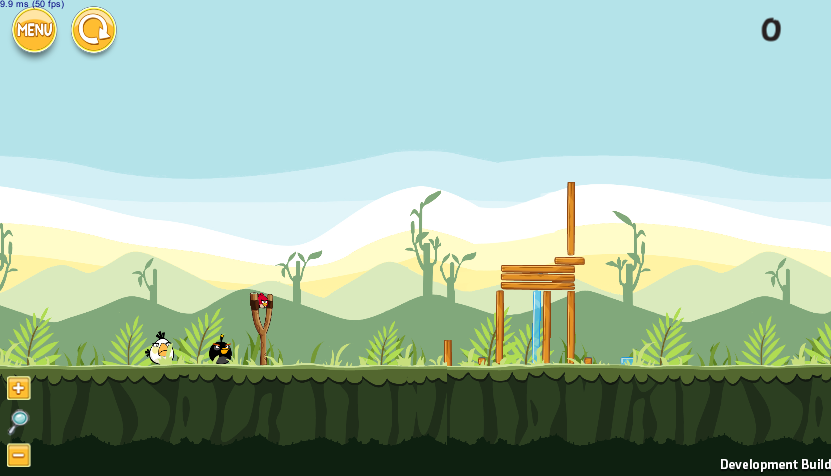
\includegraphics[scale=0.75]{E6.png}
 	\caption{One of the solutions from \ref{E6}. Blue blocks are
          composed of ice, while brownish blocks and poles are
          composed of wood. In Angry Birds, blocks differ in
          flexibility, weight but also fragility.}\label{f:e6}
 \end{figure*}


Table \ref{t:resOver1} shows that this again
increases the time needed to carry out the simulation. It also changes
the fitness landscape. Looking at Table \ref{t:resOver2}, what we
can compare mainly is the $\sigma$ and difference between best,
average and worst; fitness scores are not directly comparable since
they introduce a new term. What we see is that the variability of
solutions is decreased with respect to the previous experiment,
showing that this change increases the robustness of the algorithm,
but also its exploration capability, since the difference between the
best, worst and average is bigger than in the previous experiment. Figure \ref{f:e6} also
shows how this fitness generates structures that are stable but also
have some {\em interesting} appearance, including space that could be
occupied by pigs below the tables. At the same time, this also shows
some limitations of this approach, including the fact that three
tables are stacked one on top of each other, that there are maybe too
many poles supporting them, and that there are small blocks scattered
here and there.

The results here show that evolution is able to generate structures
that do not collapse and also have some appearance that could be
interesting. However, constraining evolution in particular ways might
lead to non-interesting structures or a local minimum in the
evolutionary landscape. Also, generated structures might be
sub-optimal in the sense that they might contain too many elements
that do not really contribute to the structure. It would be
complicated to codify this into a constraint, but it could be taken
into account in a post-processing of the structure using some greedy
algorithm.

On the other hand, this last experiment fulfills, at least partially,
the objectives of this paper: being able to find diverse,
aesthetically pleasing structures fast, without compromising, in
advance, with a specific building pattern.


%%%%%%%%%%%%%%%%%%%%%%%%%%%%%  CONCLUSIONS  %%%%%%%%%%%%%%%%%%%%%%%%%%%%
%
\section{Conclusions and Future Work} 
\label{sec:conclusions}

This paper was developed with the main objective of speeding up the
implementation of a system for generating free form Angry Birds
levels; previously, we implemented an EA that optimized stability of
generated structures, an objective that was achieved in a previous
paper. However, there were several problems with these 
structures generated initially: since their main optimization criterion was stability,
they were mostly blocks lying on the floor; this was a local minimum
and it was difficult to escape for that; additionally we needed to
submit the structure to the simulator and obtain information (such as
block speed) from it in order to evaluate those structures that
couldn't be eliminated due to constraints. In this paper we tried to
move in two different directions: incorporating a Physics engine to
the main evolutionary algorithm to minimize the need to use the
Science Birds simulator, and also try and incorporate better criteria
of structure evaluation so that they build up the kind of structures
we are used to in Angry Birds.

That is why, besides incorporating the Physics engine, which sped up
evaluation considerable and allowed us to explore a bigger space, we
took height into account in fitness, so that higher structures were
more varied and also more aesthetically pleasing. 

The main challenges ahead lie in the inherent multi-objective nature
of this problem. The fact that the structures need to be varied can be
taken into account by the very nature of the generation problem and
need not be included into fitness; this fitness should, however,
consider aesthetics. Aesthetics is part constraint (for instance,
symmetry could considered as such constraint), but also a score that
we would need to maximize. What this score could be applied to a
structure is not, a priori, straightforward. Adding to this requisite,
the level should be challenging to the user, so that it should include
a certain amount of protection for the hosted pigs, which would make
it, as hinted, a multi-objective problem. A multi-objective problem
multiplies the size of the search space, so additional speeding up
techniques should probably have to be taken into account.

If we pay attention at the stages of evolution in this work, there is also 
room for improvement in the genetic operators. For example, the initialization 
produces a small amount of valid individuals which suggested that an elitist 
strategy for selection would work best. However, new experiments will help to 
better balance exploration and exploitation. An interesting addition
would be to add {\em building} operators that pile blocks on
structures that are already stable. 

\section{Acknowledgements}
 This paper has been supported in part by DeepBio
 (TIN2017-85727-C4-2-P) from the Ministerio de Economía y Competitividad
 in Spain.

\bibliographystyle{apalike}
{\small
\bibliography{angrybirds}}

\end{document}

